\documentclass[12pt]{article}
\usepackage[utf8]{inputenc}
\usepackage{amsmath}
\usepackage{amsfonts}
\usepackage{amssymb}
\usepackage{graphicx}
\usepackage[left=2cm,right=2cm,top=2cm,bottom=2cm]{geometry}
\usepackage{wrapfig}
\usepackage{subfigure}
\usepackage{blindtext}
\usepackage{tabularx}
\usepackage{epsfig}
\usepackage{epstopdf}
\usepackage[space]{grffile}
\usepackage[nottoc]{tocbibind}
\usepackage{color}
\author{Paweł Palczyński}
\DeclareUnicodeCharacter{2212}{-}
\begin{document}

%\tableofcontents

\title{Opto-electronic properties of $WS_2$}

\maketitle

\section*{Declaration}
\section*{Acknowledgements}
\section*{Abstract}
\section*{List of abbreviations}
\section*{List of figures}
\section*{List of tables}
\section{Introduction}
	Following the discovery and characterisation of graphene in last decade the focus has been put on other 2D materials. Similar to graphene other bulk layered materials can exist in a monolayer or few layer form. Furthermore these thin layers also exhibit a significant change of properties when number of layers decreases from bulk all the way to monolayer. One of the most popular groups of these materials are transition metal dichalcogenides (TMDC). Their general form is $MX_2$ where M is a transition metal, and X is a chalcogen atom.  

	\subsection{Properties of TMDCs}
	TMDCs in their layered form have been known, studied and utilised for a long time. They can be found commonly in use as stolid-state lubricants or catalysts. About 60 different TMDCs have been studied and characterised with a general formula of X-M-X where a plane of metal atoms (M) is sandwiched between two chalcogen planes (X). Out of those 40 can be considered layered materials where individual layers are strongly bonded in-plane and weakly bonded out-of-plane in between layers. These weak, interlayer, Van der Waals interactions allow to form a bulk material. These bonds are also what allows for those layers to slide on top of one another similarly to other layered materials like graphite. 
	TMDCs consist of two transition metal and single chalcogen atoms covalently bonded. They can be found in 3 distinct structural polytypes: 1T (tetragonal symmetry, octahedral coordination) with single layer per repeat unit, 2H (hexagonal symmetry, trigonal prismatic coordination) with 2 layers per repeat unit and 3R (rhombohedral symmetry, trigonal prismatic coordination) with 3 layers per repeat unit \cite{TMDCReviewNature2012} as can be seen in Figure \ref{fig:TMDCPolytypes}.
	
	\begin{figure}[h]
	\begin{center}
	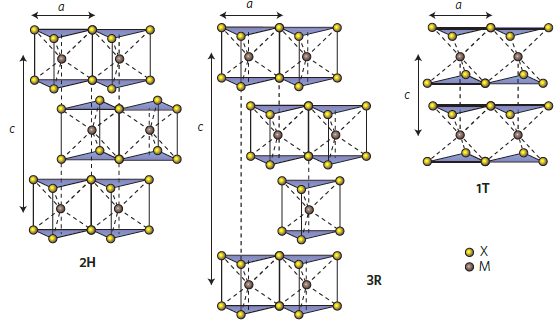
\includegraphics[scale=0.7]{TMDCPolytypes.png}
	\caption{Schematics of the structural polytypes: 2H (hexagonal symmetry, two layers per repeat unit, trigonal prismatic coordination), 3R (rhombohedral symmetry, three layers per repeat unit, trigonal prismatic coordination) and 1T (tetragonal symmetry, one layer per repeat unit, octahedral coordination). The chalcogen atoms (X) are yellow and the metal atoms (M) are grey. The lattice constants a are in the range 3.1 to 3.7 Å for different materials. Adopted from \cite{TMDCReviewNature2012}}
	\label{fig:TMDCPolytypes}
	\end{center}
	\end{figure}
	
	Since graphene have proven to be difficult to work with in the fields of semiconductors due to its lack of natural finite electronic band gap its role as a successor in electronic and opto-electronic devices remains to be seen. However the techniques learned and effects observed during its characterisation were easily transferred to other layered compounds such as TMDCs. In particular the semiconducting, group VI-based TMDCs, containing sulphur and selenium as chalocgen atoms have proven to be more readily potentially useful as an active material in electronic and opto-electronic devices. This is due to their inherent electronic and optical bandgap in visible-near IR range. 
	
	As the number of layers changes from bulk to monolayer the properties of the TMDC undergo a significant change. In most TMDCs the bandgap changes from indirect to a larger direct one. 
	
	\subsection{Electronic properties}
	\label{subsec:Electronic properties}
	
	One of the most interesting features that the layered TMDC materials exhibit is the shift in the bandstructure with the changing number of layers. Several studies have shown in simulations and experimentally that TMDCs have very similar electronic band structure as seen in example of $WS_2$ in Figure \ref{fig:WS2BandStructureSimulation}. In bulk $WS_2$ the maximum of the valence band (VBM) at $\Gamma$ point and the minimum of the conduction band (CBM) at $\Lambda$ form an indirect bandgap. As the number of the layers decreases the CBM at $\Lambda$ point as well as VBM at $K$ point increases causing the band gap to widen. At 2 layers the $K$ point becomes the actual CBM and a new indirect bandgap forms between $\Gamma$ point and $K$ point. Finally in a $WS_2$ monolayer the VBM at $K$ point as well as entire conduction band increases to form a new greater direct band gap at $K$ point. This means that $WS_2$ bandgap changes from 1.3 eV indirect bandgap in bulk to 2.1 eV direct bandgap in monolayer.
	
	\begin{figure}[h]
	\begin{center}
	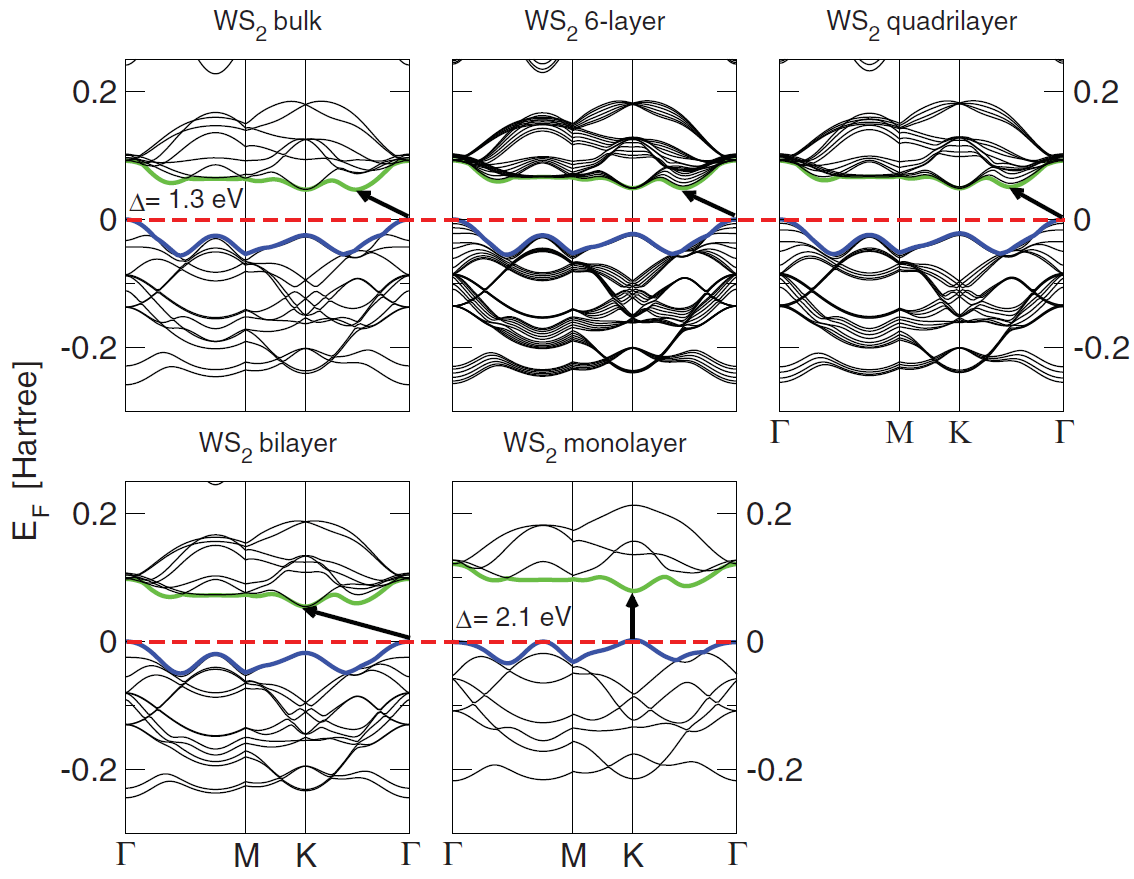
\includegraphics[scale=0.4]{WS2BandStructureSimulation.png}
	\caption{Band structures of bulk $WS_2$, its monolayer, as well as, polylayers calculated from the density functional theory (DFT) simulation. The horizontal dashed lines indicate the Fermi level. The arrows indicate the fundamental band gap (direct or indirect) for a given system. The top of valence band (blue) and bottom of conduction band (green) are highlighted. Adopted from Ref. \cite{WS2BandStructureSimulation}}
	\label{fig:WS2BandStructureSimulation}
	\end{center}
	\end{figure}
	
	Like $WS_2$ other Mo and W based TMDC undergo similar transitions as seen in Table \ref{tab:MoWBandgapsComparison}. In all cases the smaller indirect bandgap changes to greater direct bandgap with monolayer bandgap ranging from 1.1 eV to about 2.1 eV. Moreover the VBM at K points exhibits the orbit-spin band splitting at the K point of about 400 meV. This direct bandgap leads to presence of A and B excitons generated by transition between CBM and two VBMs at the K point. The conduction band as well as the valence band are dominated by the d-electron orbitals of the transition metal atoms and at the VBM and CBM they hybridize with the p-electron orbitals of the chalcogenide atoms. Because the hybridization happens mostly at the $\Gamma$ point and the chalcogenide atoms are at the surface of the TMDC layer it leads to strong interactions between the layers. This leads to significant change in the band structure at the $\Gamma$ and rise of the indirect bandgap as a result of increased number of layers. On the other hand at the $K$ point the d-orbitals of the transition metals remain mostly unaffected due to them being positioned in the middle of the layer \cite{WS2BandStructureSimulation} \cite{EmergingPhotoluminescenceInMonolayerMoS2}
	 
	 \begin{table}[h]
	 \caption{Mo and W based TMDC bandgaps comparison}
	 \label{tab:MoWBandgapsComparison}
	 \end{table}
	 
	 \begin{center}
	 \begin{tabular}{c|l|l|l}
	 
	 M$\backslash$X & $-S_2$ 			& $-Se_2$ 	& $-Te_2$\\ \hline
	 $Mo$ 			& Semiconducting	& Semiconducting	& Semiconducting	\\ 
	 				& 1L:1.8 eV			& 1L: 1.5 eV		& 1L: 1.1 eV		\\
	 				& Bulk: 1.2 eV		& Bulk: 1.1 eV		& Bulk: 1.0 eV		\\ \hline
	 W 				& Semiconducting	& Semiconducting	& Semiconducting	\\
	 				& 1L:2.1 eV			& 1L: 1.7 eV		& 1L: 1.1 eV		\\
	 				& Bulk: 1.4 eV		& Bulk: 1.2 eV		& 					\\
	 
	 \end{tabular}
	 \end{center}
	
	
	\subsection{Optical properties}
	\label{subsec:Optical properties}

	TMDCs exhibit a wide array of opto-electronic effects due to their strong light-matter effects. These effects are mostly caused by the abundant presence of excitons, bi-excitons, trions or bound excitons. As a result the change in layer thickness from bulk to monolayer alters the photoluminescence, photoconductivity and absorption in the visible to infrared range.
		
	The primary and most common quasi-particle that forms in such system is an exciton, which is a pair of a negatively charged electron and a positively charged hole bound together by Coulomb forces to form a structure similar to that of hydrogen atom. Such pair is electrically neutral and is of size exceeding size of single cell which makes it a Wannier–Mott exciton. The recombination of these excitons results in a photon emission which can be easily observed during photoluminescence characterisation. On top of excitons other quasi-particles such as trions, bi-excitons or bound excitons can be found. A trion is a group of 2 electrons and a hole or 2 holes and an electron, or otherwise described as a charged exciton. The exact nature of the trion depends usually on the type of intrinsic doping of the TMDC. A bi-exciton is a pair of excitons which is usually only observed in quantum dot systems but can be also seen in excitonically dense systems such as TMDCs. A bound exciton is similar to the free exciton but is trapped by a defect. In a typical photoluminescence spectrum several peaks can be observed depending on specific type of TMDC characterised. In $WS_2$ monolayer for instance as seen in Figure. \ref{fig:WS2TypicalPLSpectra} the strongest peak (often labelled as an A peak) at about 1.97 eV is caused by the direct transition of single-photon generated exciton. Slightly redshifted by about 30 meV from the A peak a generally weaker peak caused by the trion recombination can be found. At higher energies another peak can be observed due to the presence of bi-excitons. At around the 1.3 eV a much weaker peak (I) can be seen caused by the indirect transition. Additionally a B peak can be observed blueshifted from the A peak which is caused by valley splitting as discussed in chapter \ref{subsec:Electronic properties}. As seen in Figure \ref{fig:WS2TypicalPLSpectra} as the number of layers increases the main A peak becomes dramatically weaker due to lack of direct transition and redshifted following the pattern discussed in chapter \ref{subsec:Electronic properties}. At the same time the I peak becomes relatively stronger and eventually dominates the bulk material.
		
	\begin{figure}[h]
	\begin{center}
%	\includegraphics[scale=1]{•}
	\caption{Typical PL spectra of $WS_2$}
	\label{fig:WS2TypicalPLSpectra}
	\end{center}
	\end{figure}
		
	Similarly the photoconductivity of the TMDCs is strongly reliant on the number of layers and incident photon energy. The $MoS_2$ for instance shows 3 times stronger photoconductivity in monolayer around 1.8 eV, where the direct transition is located, than in 2L $MoS_@$ around 1.6 eV. Additionally the photoconductivity appears to increase in steps with relation to the photon energy following the direct and indirect transitions. \cite{ElectronicsAndOptoelectronicsOfTwo-dimensionalTransitionMetalDichalcogenides}.
		
	The sunlight absorption in TMDCs has been shown to be significantly more intense than in commonly used solar cell materials, at about 5-10$\%$ which is an order of magnitude greater compared to similar thickness of Si or GaAs. It is also stronger compared to 2-3$\%$ of sunlight absorption of graphene. As a result a excitonic solar cell based on $MoS_2/WS_2$ bilayer shows about 1$\%$ power efficiency, about 3 times greater than that of typical ultrathin solar cells \cite{ExtraordinarySunlightAbsorptionAndOneNanometerThickPhotovoltaicsUsingTwo-DimensionalMonolayerMaterials}.
	
	During standard single photon excitation photoluminescence studies the excitons generated can be called "bright" since they appear in PL spectrum. The reason we can observe them easily is because the spin between an electron and a hole is conserved, and thus allowing for photon emission. However another combination is possible, called dark exciton, where both electron and the hole have the same spin. Because of that they cannot recombine by emitting a photon and therefore remain absent from the PL spectrum. Even though they exist much longer than their bright counterparts their presence is of course also more difficult to observe. One way to observe them is to use two photon excitation. Due to two photon selection rule the single photon excitation can be excluded and the dark excitonic states can be observed. In WS2 the dark excitons result in two peaks at 2.28 eV and 2.48 eV. [Probing excitonic dark states in single-layer tungsten disulphide]
	
	Defect engineering allows to tune the number of charge carriers. In MoS2 or WS2 the sufur vacancies lead to increased number of electrons in the material. Because of that by increasing the number of defects in those materials the level of n-doping can be changed. An easy way to observe the presence of those defects and subsequent quenching of them is to expose the material to varying amounts of oxygen, nitrogen or water. Due to greater electronegativity (???) those species attract the electrons and therefore the electron population in the material decreases. This in turn leads to smaller trion population since trions require an extra electron to form. This then can be observed in PL as a more narrow direct peak, with especially smaller redshifted shoulder. The effect can also be of course reversed by decreasing the amount of oxygen, nitrogen or water in the environment since those exist in already in ambient conditions [Optical control of charged exciton states in tungsten disulfide].
	
	In order to introduce and control the amount of vacancies in the TMDC different method have to be explored. One of the ways of achieving that in already grown material is the use of oxygen plasma. It has been shown that the number of defects can be controlled by limiting the plasma exposure. During the process the oxygen also chemically bonds to the MoS2 at the defect sites and therefore partially negates the effect of defects on the optical properties. The PL can also be seen to increase in intensity with increasing number of defects with oxygen adsorped due to the increased yield of bound excitons localised at these defects. [Strong Photoluminescence Enhancement of MoS2 through Defect Engineering and Oxygen Bonding]
	
	Similar effect has been shown using the 2,3,5,6-tetrafluoro-7,7,8,8-tetracyanoquinodimethane ($F_4TCNQ$), 7,7,8,8-tetracyanoquinodimethane ($TCNQ$) and (nicotinamide adenine dinucleotide) $NADH$ for chemical doping. Both $F_4TCNQ$ and $TCNQ$ are p-type dopants while $NADH$ is a n-type dopant. By exposing the surface of MoS2 to these compounds the change in PL intensity and FWHM have been observed. Similar to doping with $O_2$, $N_2$ or $H_2O$, all of which are p-type dopants, the intensity of PL has increased in presence of $F_4TCNQ$ and $TCNQ$. The effect has been similarly ascribed to lowering the number of defects and therefore the lowering the trion population and subsequently increasing the exciton population increasing the yield. The opposite observation has been made with use of $NADH$ with PL intensity decreasing. Similarly the increase in trion population with lower PL yield is ascribed to the lower PL intensity. [Tunable Photoluminescence of Monolayer MoS2 via Chemical Doping].
	
	It has also been show that alloying can be used to fine tune the PL by varying the concentration of alloying material. In monolayer $Mo_{1-x}W_xS_2$ the PL peak position initially decreases from 1.575 eV (PL peak position of pure MoS2) to 1.56 eV at x=0.21 and then increase up to 1.65 eV (PL peak position of WSe2) at x = 1. This effect could be attributed to the linearity of VB and non-linearity of CB with regards to change in W composition. The PL position can therefore be engineered on a monotonic range from 1.56 eV to 1.65 eV. In bilayer $Mo_{1-x}W_xS_2$ alloy the position of both direct and indirect transition PL peaks increases monotonically from about 1.49 eV and 1.53 eV for pure MoSe2 to 1.56 eV and 1.62 eV for pure WSe2 as the W amount is increased. This opens another relatively easy way of engineering PL position [Two-Dimensional Molybdenum Tungsten Diselenide Alloys: Photoluminescence, Raman Scattering, and Electrical Transport].
	
	Another effect that has been demonstrated that allows for certain degree of control of PL in TMDCs is relation between the helicity of incident light and valley population valley population. It has been shown that by exciting the monolayer $MoS_2$ with right-polarised light the resulting excitons will fill primarily the VB at K point. Similarly by exciting the $MoS_2$ with left-polarised light the excitons will fill the VB at K' point. After recombination the resulting photons will exhibit the same circular polarity as the photons that excited the electrons in the first place. [Tightly bound trions in monolayer MoS2] [Control of valley polarization in monolayer MoS2 by optical helicity]
	
	The temperature effect on TMDCs has also been investigated. In $WSe_2$ monolayer it has been shown that as the temperature of the sample increases from room temperature to about 400K the position of the direct transition PL peak redshifts from about 1.65 eV to about 1.58 eV. When the temperature is decreased from room temperature to about 5K the same peak blueshifts to about 1.7 eV. Between 100K and 50K as well 20K and 5K the position of the PL peak does not change. Additionally around 120K another peak appears and as the temperature is lowered it also blueshifts although less than the RT peak. The peak only present at RT is attributed to free excitons whereas the peak appearing at 120K is ascribed to bound excitons. As bound exciton peak appears its intensity increasese with lower temperature while the intensity of the free exiton peak decreases. This indicates that the population of free excitons decreases while the population of the bound excitons increases with decreasing temperature \cite{PhotoluminescencePropertiesAndExcitonDynamicsInMonolayerWSe2}
	
	There has been many reports on the spatial distribution of PL in the TMDCs. One of the observed patterns in WS2 and MoS2 has been that of much stronger PL intensity at the edges of the flakes. That effect has been primarily observed in small flakes of about 5 $\mu m$ \cite{ExtraordinaryRoomTemperaturePhotoluminescenceInTriangularWS2Monolayers}.
	
	\subsection{Phonon dispersion}
	
	The vibrational and phononic characteristics of TMDCs have been investigated at length by both theoretical simulations as well as experimental studies. The $2H-MX_2$ crystal structure of the TMDCs belongs to $D_{6h}^4$ point group and there are 18 lattice dynamical modes at the $\Gamma$ point. Phonons belonging to these modes can be represented as Eq. \ref{eq:PhononDispersionRepresentation} \cite{LatticeDynamicsInMono-AndFew-LayerSheetsOfWS2AndWSe2}: 
	
	\begin{equation}
	{\Gamma} = A_{1g} + 2A_{2u} + B_{1u} + 2B_{2g} + E_{1g} + 2E_{1u} + E_{2u} + 2E_{2g}
	\label{eq:PhononDispersionRepresentation} 
	\end{equation}
	
	In TMDCs 4 active Raman modes can be observed $E_{1g}, E^1_{2g}, E^2_{2g}, A_{1g}$. These can be seen in Figure \ref{fig:4ActiveRamanModes}. The $E^2_{2g}$ is a shear mode that involves 2 layers vibrating against each other. The $E_{1g}$ is an in-plane vibration of chalcogen atoms but is forbidden in the back-scattering configuration. For monolayers therefore it leaves primarily the $E^1_{2g}$ which is an in-plane mode involving vibration of both metal and chalcogen atoms as well as $A_{1g}$ which is an out-of-plane mode involving only chalcogen atoms. 
	
	\begin{figure}[h]
	\begin{center}
	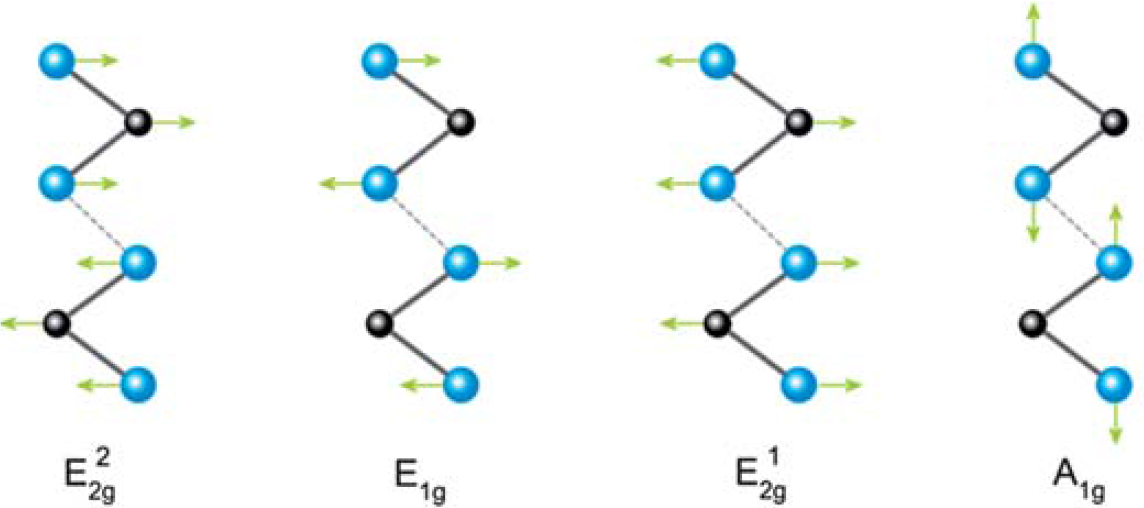
\includegraphics[scale=0.4]{RamanActiveModes.png}
	\caption{4 active Raman modes in TMDCs. Metal atoms and chalcogen atoms are black and blue respectively. Adopted from \cite{LatticeDynamicsInMono-AndFew-LayerSheetsOfWS2AndWSe2}}
	\label{fig:4ActiveRamanModes}
	\end{center}
	\end{figure}
	
	These two peaks tend to dominate the spectrum of any TMDCs, whether monolayer or few-layer or bulk. The shear mode $E^2_{2g}$ appears at low Raman shift frequencies and is therefore difficult to observe but can be used to differentiate monolayer from few-layer material. Since $E^1_{2g}$ is an in-plane mode it tends to be unaffected by the number of layers due to weak van der Vaals forces between the layers but can be seen to be slightly redshifted as the number of layers increases. As seen in Figure \ref{fig:TypicalRamanSpectrumWS2} the $E^1_{2g}$ peak at about 352 $cm^{-1}$ is overlapping with another stronger peak, a 2LA(M) peak at 350 $cm^{-1}$ which is a longitudinal acoustic mode caused by in-plane collective oscillations of W and S atoms. The second strongest peak at around 416 $cm^{-1}$ is an $A_{1g}$ peak, caused by out of plane vibrations. Because of that it is much more sensitive to the number of layers and is seen to become blueshifted as the number of layers increases. This has been attributed to the restorive forces as well as increase in dielectric screening of the Coulomb forces. Combining both of these shifts in frequency with the changing number of layers the difference between these two peak position can be used to identify the number of layers in TMDCs as seen in Figure \ref{fig:LayerNumberIdentificationRamanShiftWS2}
	
	\begin{figure}[h]
	\begin{center}
%	\includegraphics[scale=1]{•}
	\caption{Typical Raman spectrum of $WS_2$}
	\label{fig:TypicalRamanSpectrumWS2}
	\end{center}
	\end{figure}
	
	\begin{figure}
	\begin{center}
%	\includegraphics[scale=•]{•}
	\caption{Identification of number of layers by the difference in position of $A_{1g}$ and $E^1_{2g}$ peaks.}
	\label{fig:LayerNumberIdentificationRamanShiftWS2}
	\end{center}
	\end{figure}
	
	\subsection{Heterostructures}
	\subsection{Applications}
\section{Methods}
	\subsection{Raman spectroscopy theory}
	\subsection{Photoluminescence spectroscopy theory}
	\subsection{XPS theory}
\section{Characterisation of $WS_2$}
	\subsection{Optical microscopy of $WS_2$ flakes}
	\subsection{Raman spectroscopy of $WS_2$}
		\subsubsection{Interlayer interactions}
		\subsubsection{Strain}
		\subsubsection{Grain boundaries}
	\subsection{Photoluminescence spectroscopy}
		\subsubsection{PL of $WS_2$ monolayer}
		\subsubsection{PL variation vs flake size}
		\subsubsection{PL variation vs synthesis conditions}
		\subsubsection{Spatial PL variation}
		\subsubsection{Effects of water and oxygen on PL}
\section{Transfer of mono- and fewlayer $WS_2$}
	\subsection{Motivation}
	\subsection{Wet transfer}
		\subsubsection{Methods}
		\subsubsection{Effects on optical and electronic properties}
	\subsection{Dry transfer}
		\subsubsection{Methods}
		\subsubsection{Effects on optical and electronic properties}
\section{Low temperature characterisation of $WS_2$}
	\subsection{Setup}
	\subsection{Isolating trions and excitions}
	\subsection{Spatial variation of PL}
\section{In doped $WS_2$}
	\subsection{Doping theory}
	\subsection{Quantifying In doping}
	\subsection{Effects of doping on PL}
	\subsection{Effects of doping on Raman spectroscopy}
\section{Heterostructures}
	\subsection{Introduction}
	\subsection{Synthesis}
	\subsection{Raman and PL characteristics}
\section{Applications}
	\subsection{Transistors}
	\subsection{LEDs}
	\subsection{Transparent electrodes}
	
\section*{References}
\section*{Appendix}

\section*{Publications}

F. Reale \textit{et al}, "High-Mobility and High-Optical Quality Atomically Thin $WS_2$" Scientific Reports, 2017 - submitted\\ \\
F. M. Pesci \textit{et al}, "MoS2/WS2 heterojunction for photoelectrochemical water oxidation", ACS Catalysis, 2017 - accepted

\section*{Conferences}

Graphene Week, 13-17 June, 2016. (Best poster)\\ \\
UK Semiconductors, 14-15 July, 2017.\\ \\
MRS Boston, 26 November - 1 December, 2017.

\bibliographystyle{plain}
\bibliography{bibliography}{}

\end{document}